\chapter{Background}\label{chapter:background}

This section aims on providing a general overview of the various tools that were used in this work. In particular, the employed edge devices as well as the FaaS platform that was chosen to construct the experimental cluster will be introduced.

\section{Cluster Monitoring \& Data Visualization}
\subsection{Prometheus}
\textit{Prometheus} is an Open-Source, cutting-edge monitoring system that enables administrators to effectively supervise a system's infrastructure and associated applications. It is well known for its poll-based data collection model which regularly scrapes metrics over HTTP from the services being monitored, which are usually referred to as \textit{targets}, using a configurable time interval. Any data collected by a successful scrape is stored in a time-series database, which enables Prometheus to keep track of changes of the individual metrics over time. For the purpose of data selection and performing operations on the data, Prometheus provides an own query language called \textit{PromQL} which defines a wide range of functions that can be utilized in query expressions. Furthermore, it allows to define certain alert rules that are based on the collected data in order to trigger an alert once a specific condition defined in those rules is met. This allows for sending automatic notifications to administrating staff, which can then act appropriately based on what kind of alert has been triggered.\\
Generally, there is already a comprehensive amount of applications that natively expose metrics in the format expected by Prometheus. For any cases where this does not apply, a so-called data exporter can be employed, which is responsible for fetching data from third-party systems and transforming them into metrics that can be processed by Prometheus. To this end, client libraries that are available for a variety of programming languages can be made use of in order to implement such an exporter for a specific application.

\subsection{Grafana}
\textit{Grafana} is a modern Open-Source data analytics \& visualization platform that offers the possibility to plot data, which can be obtained from a variety of different sources, in interactive, dynamic dashboards. Prometheus is one of the most commonly used data sources for Grafana, which qualifies it as another powerful component of a modern system monitoring toolchain. Due to the fact that it provides the opportunity to construct an arbitrary amount of dashboards that are highly configurable, users are able to achieve a visualization of their data that satisfies individual requirements.


\section{Edge-Enabled IoT Devices}

\subsection{Raspberry Pi 3 A+}

\begin{figure}[h]
    \centering
    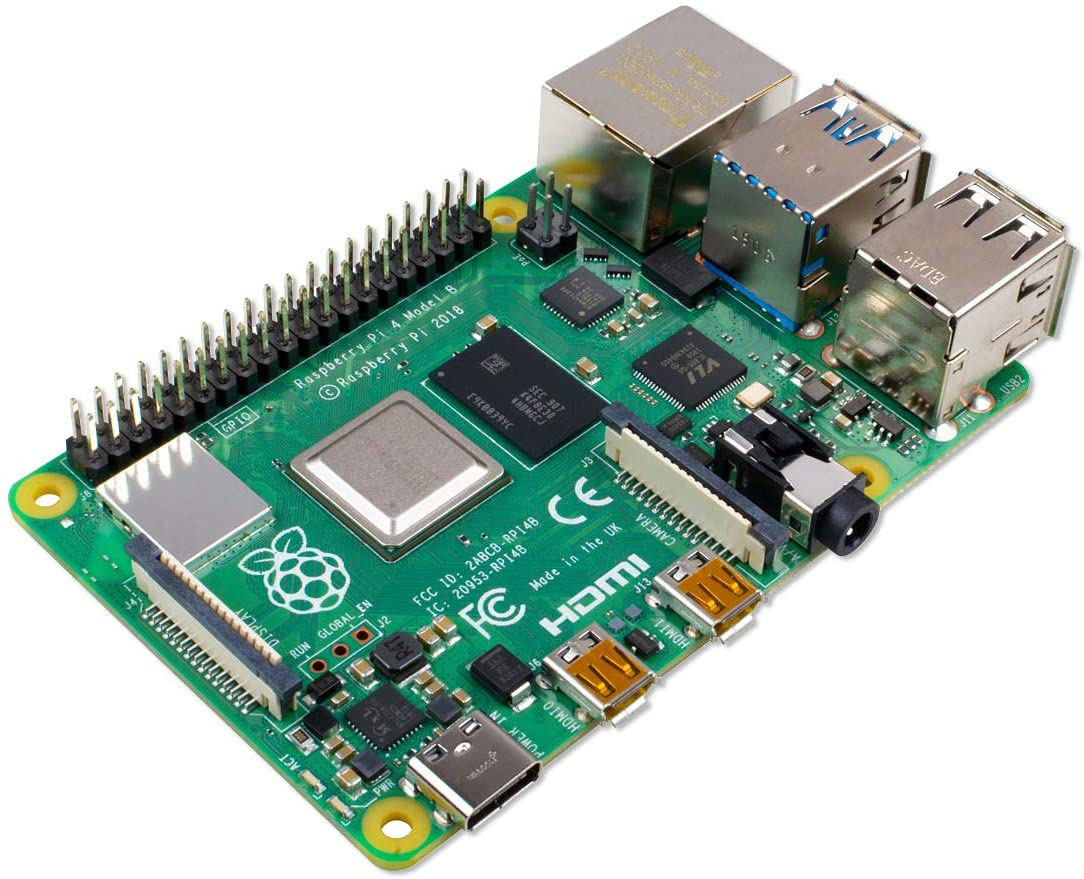
\includegraphics[width=0.30\textwidth]{./figures/mesh}
    \caption{The Raspberry Pi 3 A+}
    \label{fig:raspberry-pi}
\end{figure}


The Raspberry Pi 3 A+ is the third generation model of the probably most commonly known single-board computer - the Raspberry Pi. It was developed by the british Raspberry Pi Foundation and is equipped with 1 GB of RAM and a Cortex-A53 Quad-Core ARM64 processor that operates at 1.2 GHz. It demands a power supply of 5V at 2.5A in order to be operated.

\subsection{NVIDIA Jetson Nano Developer Kit}

\begin{figure}[h]
    \centering
    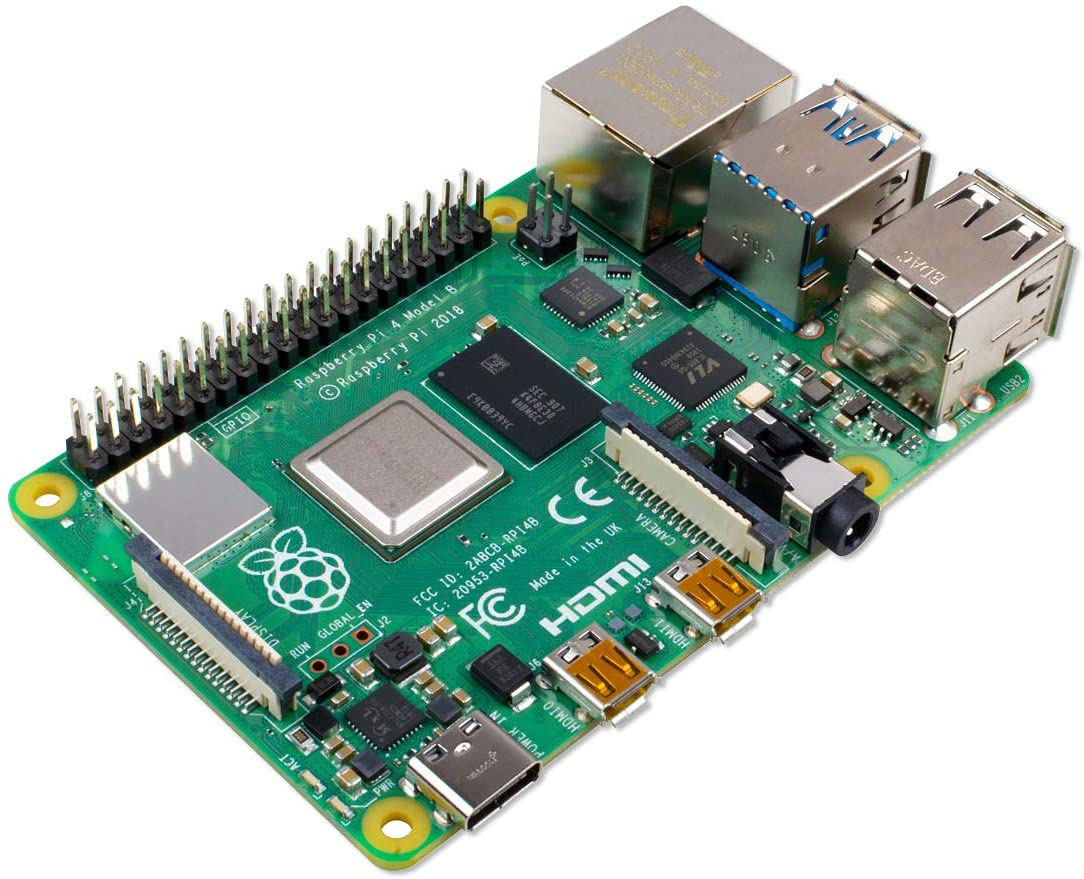
\includegraphics[width=0.30\textwidth]{./figures/mesh}
    \caption{The NVIDIA Jetson Nano Developer Kit}
    \label{fig:jetson-nano}
\end{figure}

The NVIDIA Jetson Nano Developer Kit is a performant single-board computer developed by the NVIDIA Corporation and is primarily designed for the purpose of developing and executing AI applications. To this end, it is provided with a Cortex-A57 Quad-Core ARM64 CPU that runs at 1.43 GHz as well as with an NVIDIA 128-core NVIDIA Maxwell GPU. Additionally, the Jetson Nano Developer Kit has access to 4 GB of LPDDR4 RAM and requires a slightly higher power supply of 5V at 2.5A - however, supplying up to 4A is recommended.~\parencite{jetson-nano-devkit-manual}

\subsection{Google Coral Dev Board}

\begin{figure}[h]
    \centering
    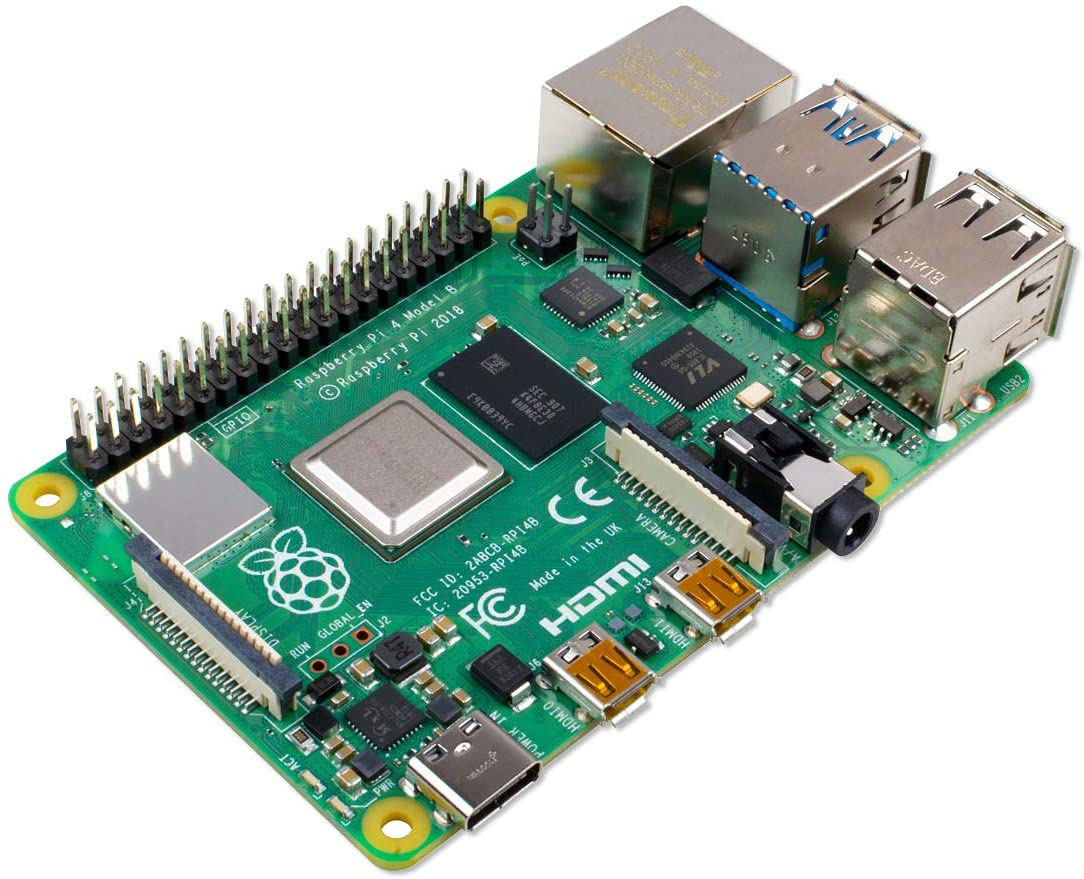
\includegraphics[width=0.30\textwidth]{./figures/mesh}
    \caption{The Google Coral Dev Board}
    \label{fig:coral-dev-board}
\end{figure}

The Coral Dev Board is a single-board computer designed to facilitate machine learning inference and embedded system development. Next to a Vivante GC7000Lite GPU and a Cortex-A53 Quad-Core ARM64 processor that operates at up to 1.5 GHz, it is equipped with an Edge TPU coprocessor developed by Google which significantly leverages the performance. Moreover, it is provided with 1 GB of LPDDR4 RAM and demands a power supply of 5V at around 2-3A.~\parencite{coral-dev-board-manual}

\subsection{Odroid XU4}

\begin{figure}[h]
    \centering
    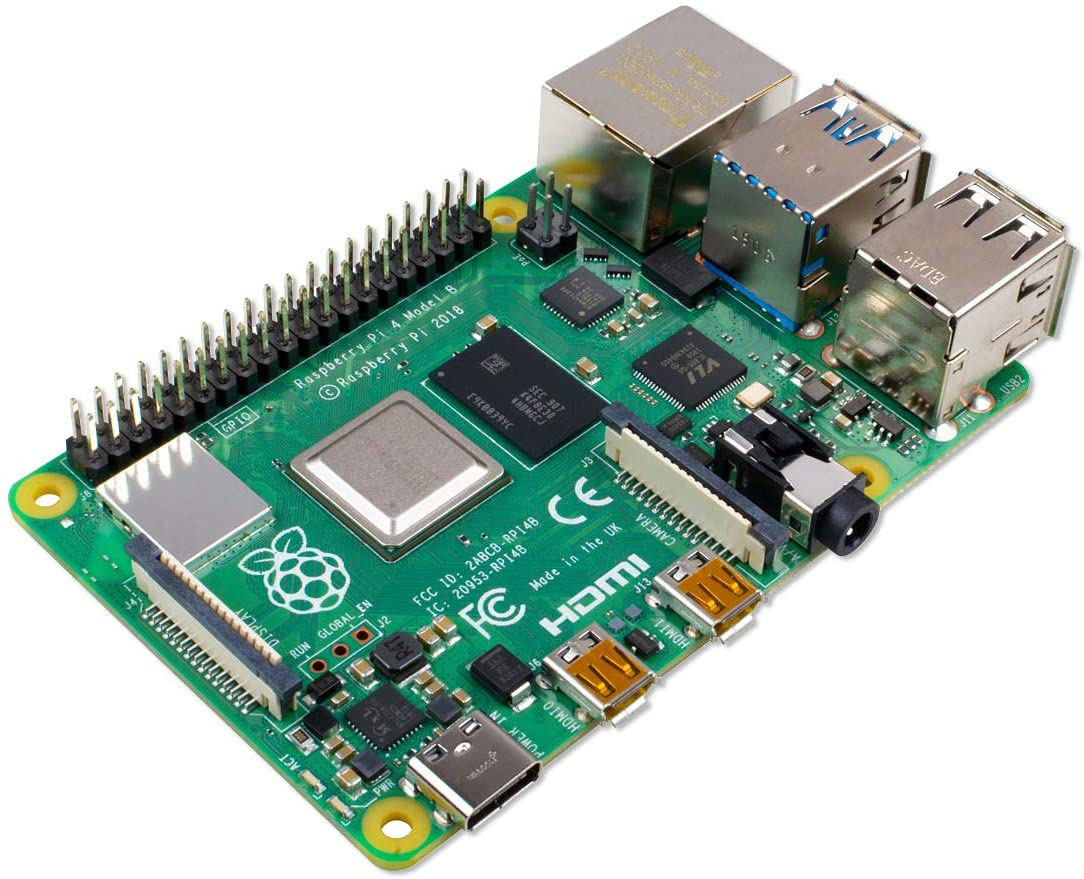
\includegraphics[width=0.30\textwidth]{./figures/mesh}
    \caption{The Odroid XU4}
    \label{fig:odroid-xu4}
\end{figure}

The ODROID XU4 is a powerful single-board computer manufactured by Hardkernel, which is specifically well suited for developing software designed for the android operating system. It comes with a SAMSUNG Exynos 5422 Octa-Core ARM CPU running at 2 GHz, an integrated Mali-T628MP6 GPU and 2 GB of LPDDR3 RAM. Even though the board consumes less than 1A in the most cases, providing a power source supplying 5V at 4A is recommended in order to operate the XU4.~\parencite{odroid-xu4-manual}

\subsection{XILINX PYNQ-Z1}

\begin{figure}[h]
    \centering
    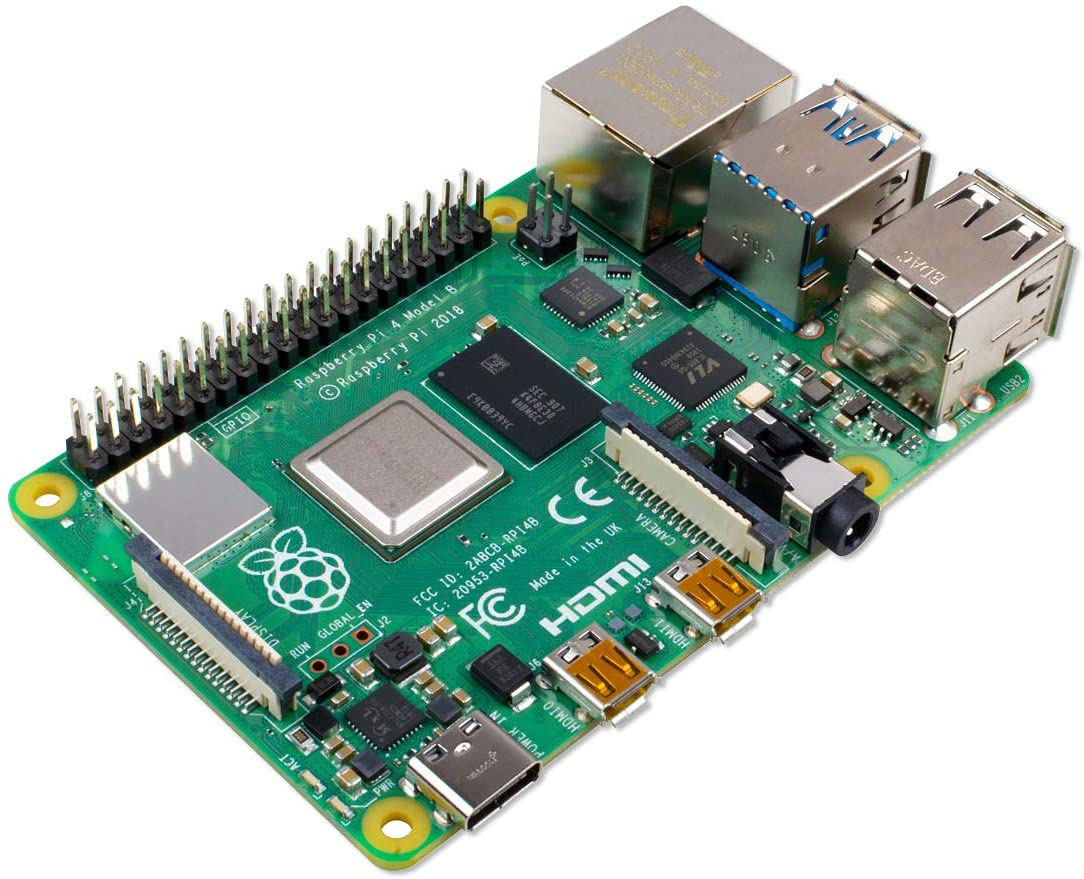
\includegraphics[width=0.30\textwidth]{./figures/mesh}
    \caption{The XILINX PYNQ-Z1}
    \label{fig:xilinx-pynq-z1}
\end{figure}

The XILINX PYNQ-Z1 is a general purpose single-board computer manufactured by Digilent. It is designed to be used with the Open-Source framework PYNQ, which is based on the programming language Python and facilitates prototyping and embedded software development for the individual XILINX platforms. The board is supplied with 512MB of DDR3 RAM and a Cortex-A9 Dual-Core processor which operates at up to 650 MHz. At the bare minimum, the PYNQ-Z1 can be powered via USB 2.0, which, according to the specifications, provides 5V at up to 0.5A. For more complex applications, an external source supplying 7V at the minimum and 15V at the maximum should be used~\parencite{pynq-z1-manual}.

\section{OpenFaaS}

\begin{figure}[h]
    \centering
    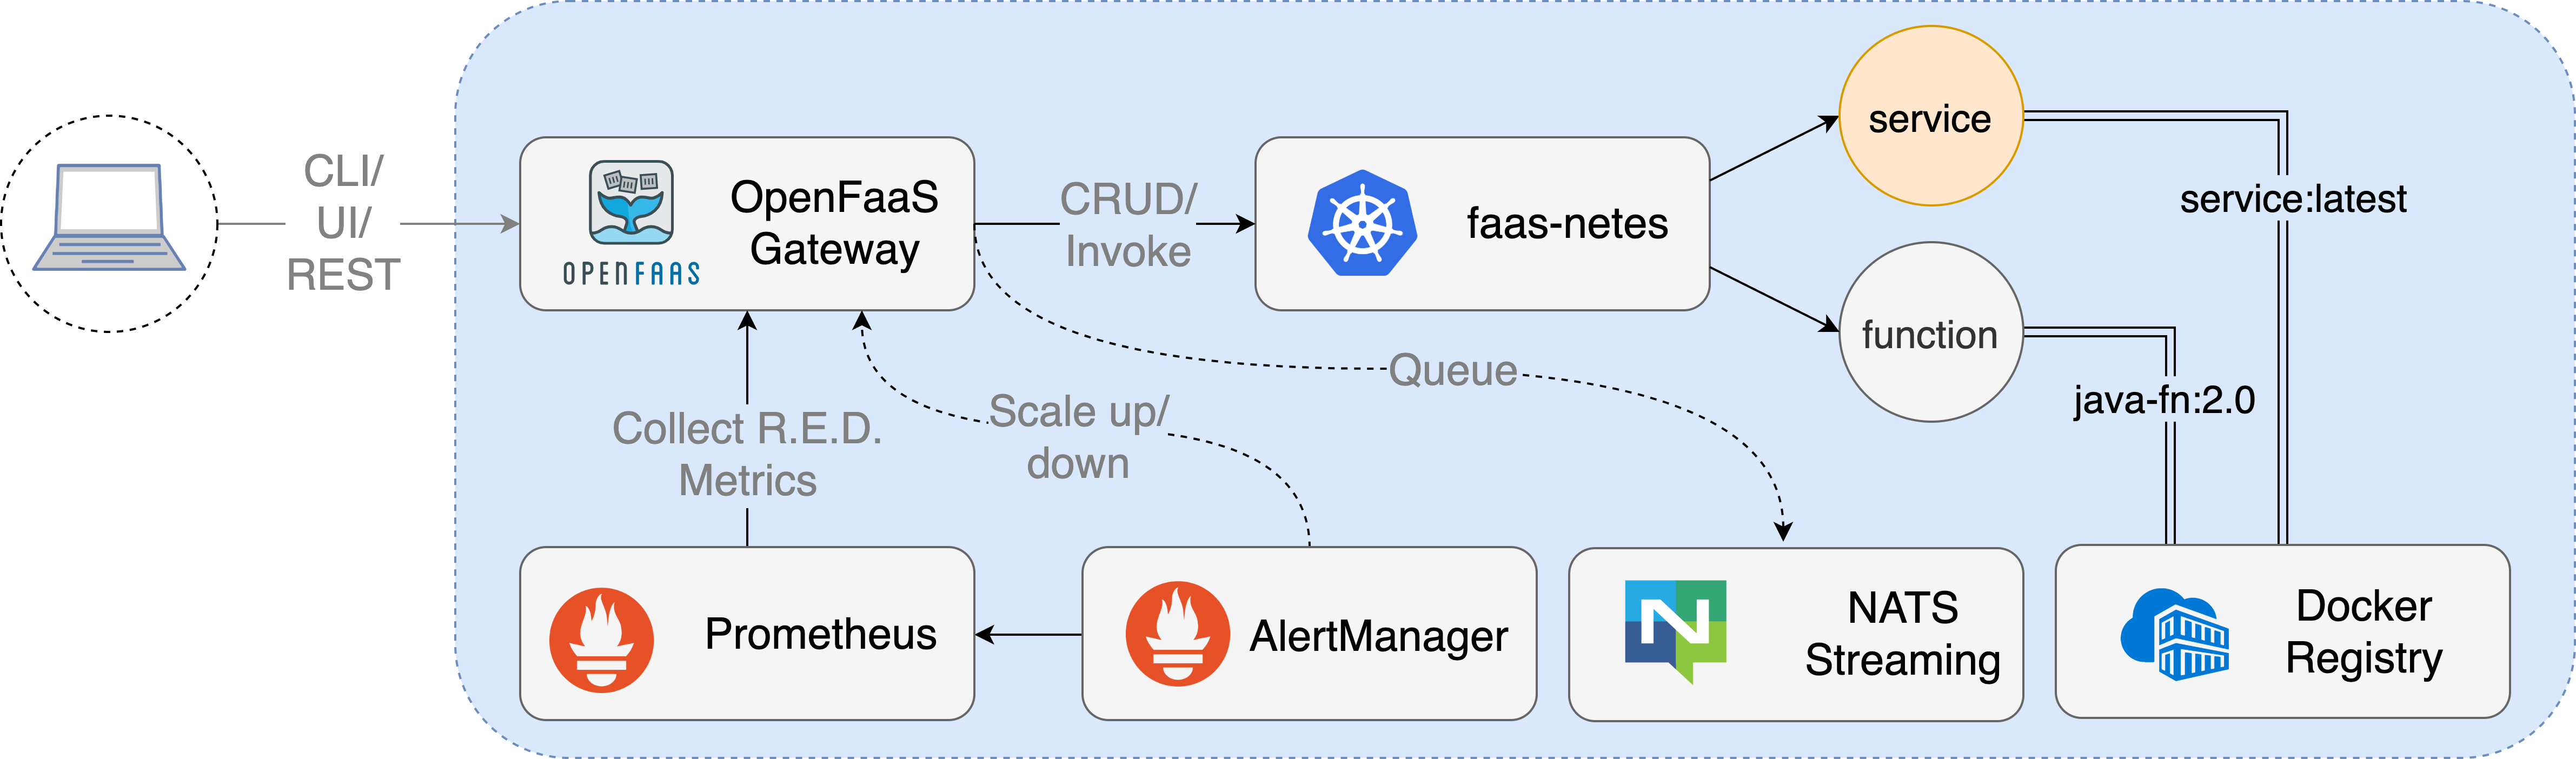
\includegraphics[width=1\textwidth]{./figures/of-workflow.png}
    \caption{Interaction with the OpenFaaS API Gateway~\parencite{openfaas-stack}}
    \label{fig:openfaas-gateway}
\end{figure}

OpenFaaS is one of the most popular Open-Source FaaS platforms and is suitable for production-ready, large-scale applications as well as for less complicated projects due to the fact that it either can be deployed to the commonly known industrial-strength container orchestration systems Kubernetes and OpenShift or to faasd, which offers the opportunity to avoid the complexity of the aforementioned tools \parencite{openfaas-deployment}. Serverless functions for OpenFaaS can be written in any programming language as the only requirement is packaging the application as a container image that complies with the OCI format and publishing it to an image registry, which makes it very straightforward and easy to use~\parencite{openfaas-intro}. The deployed serverless functions are invoked by the \textit{OpenFaaS API Gateway} which can be accessed via its REST API, the provided Command Line Interface (CLI) or the Web UI. Moreover, invocations can be triggered by a scheduled cron-job or a multitude of events such as notifications from message brokers like \textit{Apache Kafka} or \textit{RabbitMQ}~\parencite{openfaas-triggers}. Figure 2.6 provides an overview of the overall collaboration of the individual components that are involved during the invocation of a function in OpenFaaS.

\section{Function Delivery Network}
Current FaaS platforms are restricted to homogeneous clusters and serverless functions, which is a significant limitation due to the fact that heterogeneity of compute clusters and computational resources is steadily increasing in today's cloud applications. For instance, an IoT application may utilize an IoT cloud that consists of a cluster of multiple microcontroller-based systems, which might use different processor architectures and substantially differ in their hardware equipment, and another cluster composed of powerful Virtual Machines (VMs), which is responsible for handling the computationally more intensive tasks. Consequently, serverless functions that demand a significant amount of compute and data resources should be scheduled in an appropriate cluster that is able to fulfill these requirements. Additionally, it is important to mention that, due to hardware constraints present on edge devices, it can not be guaranteed that a certain FaaS platform can actually run on them, which prevents the use of a homogeneous FaaS platform over multiple heterogeneous clusters ~\parencite{fdn}.
In summary, this implies the need for the possibility to deploy heterogeneous FaaS platforms in heterogeneous clusters and to schedule the execution of serverless functions based on their individual resource requirements. To this end, data access behavior such as access latency should be taken into account in an effective manner in order to optimally utilize the available resources.
\\
The Function Delivery Network (FDN) is a distributed network of target platforms, which is designed to extend the concept of serverless computing based on FaaS in order to overcome the mentioned limitations. It is highly versatile as it can be integrated with a wide range of different target platforms. The FDN supports clusters dedicated for a multitude of purposes such as cloud and edge computing as well as High Performance Computing (HPC) and can be used with multiple FaaS providers like Apache OpenWhisk, OpenFaaS, AWS Lambda or Google Cloud Functions.\\
It supplies FDaaS by requiring the user to provide an application configuration file, which describes the individual functions, APIs, permissions and other associated configuration. This file is subsequently passed to the following core components of the FDN:

\begin{enumerate}
    \item \textit{Deployment Generator}: This unit annotates the file with a deployment configuration for the specific application based on knowledge that was either previously collected by the FDN or externally provided by an expert.
    \item \textit{Control Plane}: This is the main component of the FDN. It is responsible for managing the access control which includes authentication and authorization as well as for monitoring the overall infrastructure and applications. Additionally, it handles data placement and the scheduling of function invocations based on the annotated deployment specification.
\end{enumerate}

The decisions regarding function scheduling and data placement made by the Control Plane at runtime depend on several behavioral models, which are created by another component called  \textit{Behavioral Modeling} during the execution of an application. These models are continuously updated in an online learning fashion by extracting knowledge from data that is regularly collected by the FDN from the application's functions ~\parencite{fdn}.